%================================================================
\section{Appendix}\label{sec:Appendix A}
%================================================================

%----------------------------------------------------------------
\subsection{Additional Results}\label{app:additional_results}
%---------------------------------------------------------------- 


% hh_mse_kld_vs_beta_conv_vae.pdf

\autoref{fig:hh_conv_vae_beta_0_5} and \autoref{fig:hh_conv_vae_beta_2} are supplementary to \autoref{fig:hh_conv_vae_beta_1_z_20} and \autoref{fig:hh_conv_vae_beta_1_z_2_10}, and show the convolutional $\beta$-VAE's reconstructed and generated voltage traces for $\beta = 0.5$ and $\beta=2$, respectively, with $\dim (z) = \{2, 10, 20\}$.

\begin{figure}[!htb]
\centering
\subfloat[]{{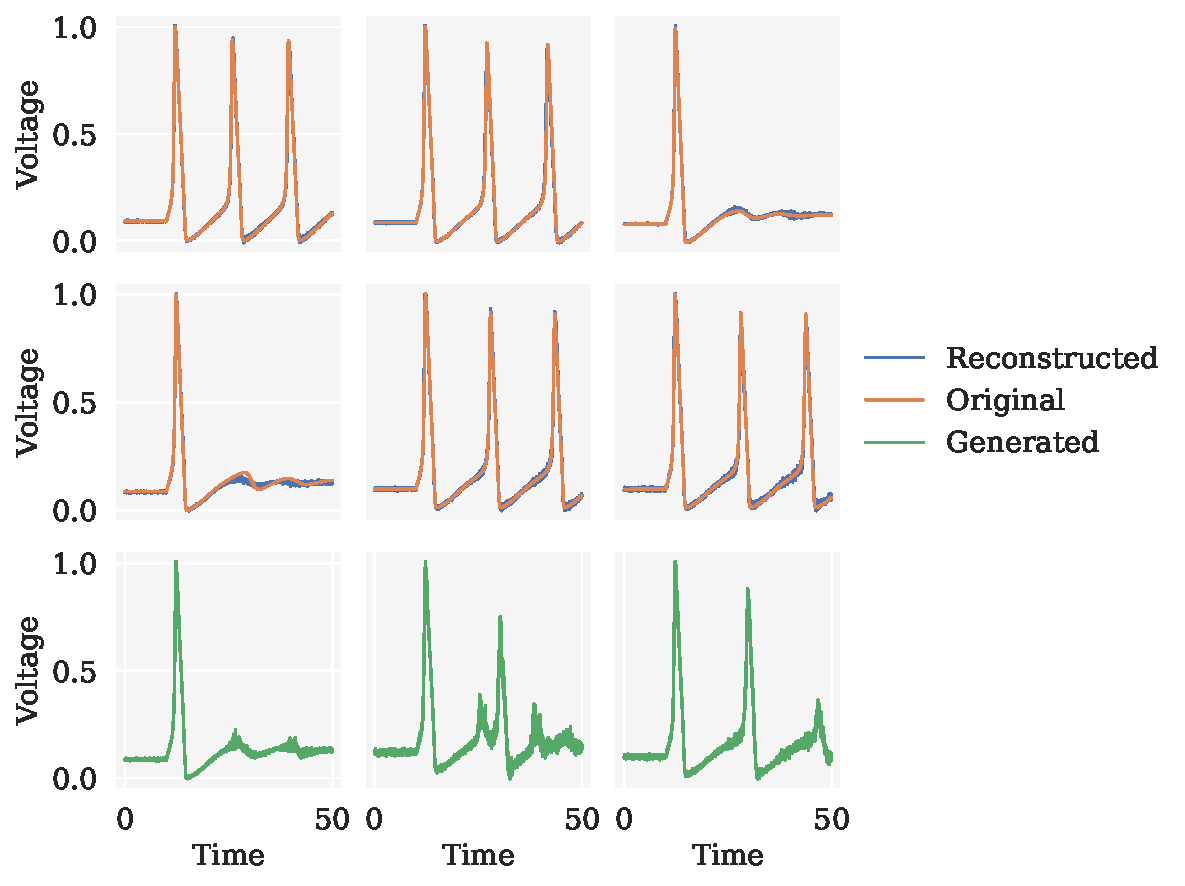
\includegraphics[scale=0.38]{latex/figures/hh_conv_vae_beta_0.5_z_2.pdf}}}
\qquad
\subfloat[]{{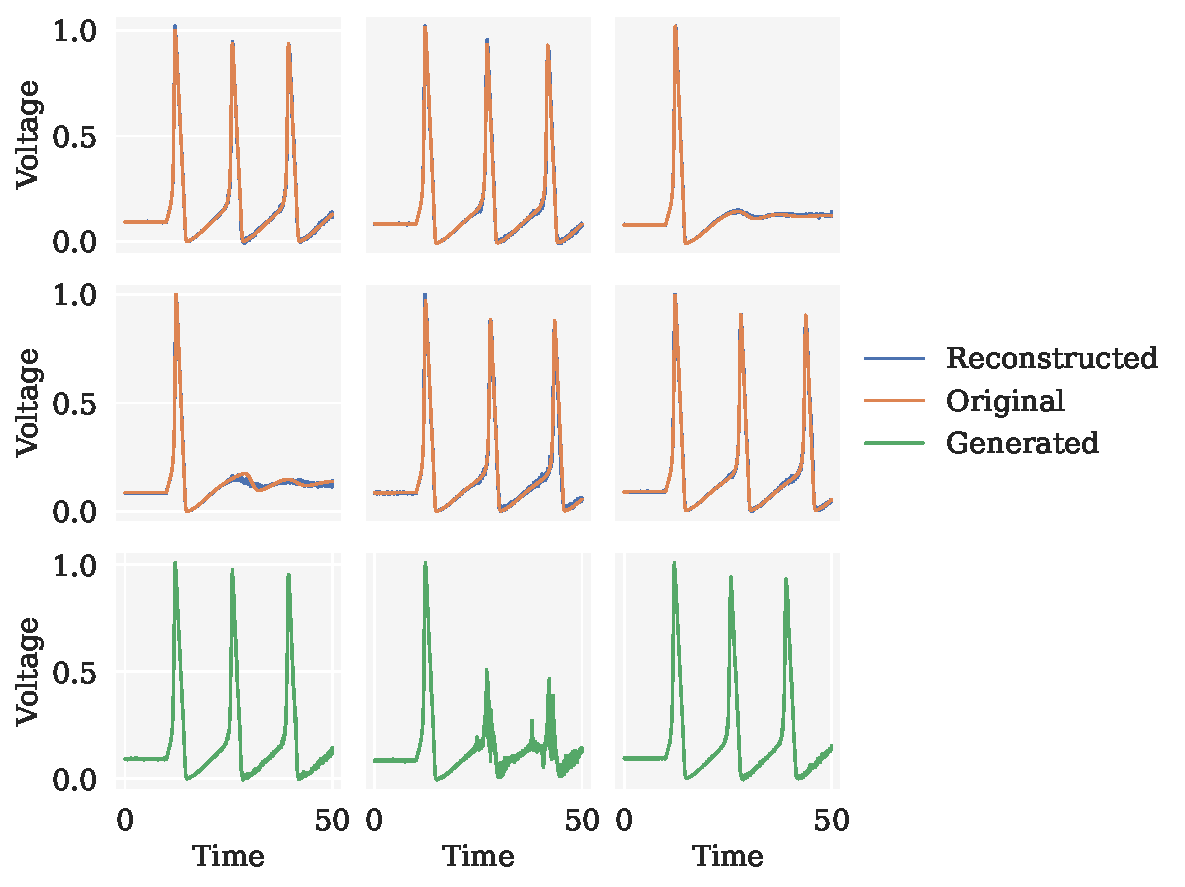
\includegraphics[scale=0.38]{latex/figures/hh_conv_vae_beta_0.5_z_10.pdf}}}
\qquad
\subfloat[]{{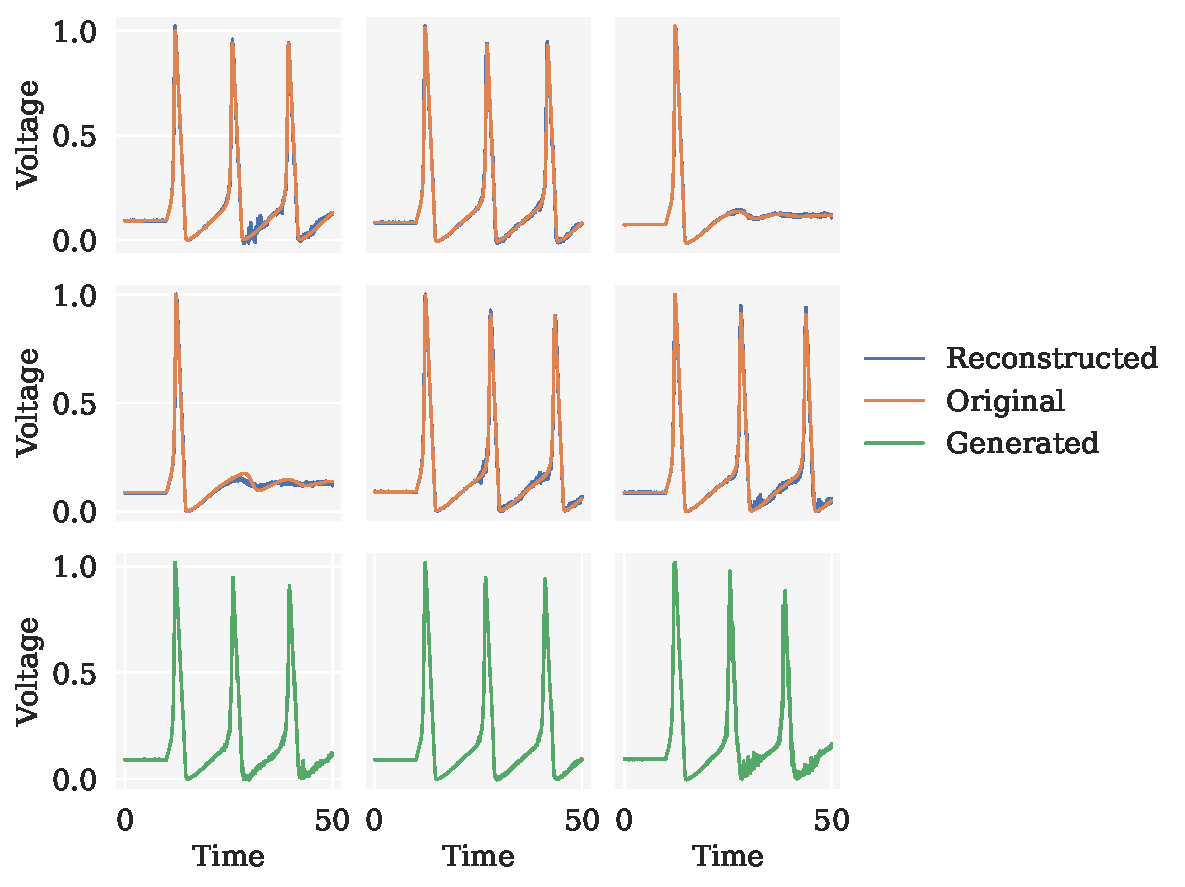
\includegraphics[scale=0.38]{latex/figures/hh_conv_vae_beta_0.5_z_20.pdf}}}
\caption{beta 0.5}
\label{fig:hh_conv_vae_beta_0_5}
\end{figure}

\begin{figure}[!htb]
\centering
\subfloat[]{{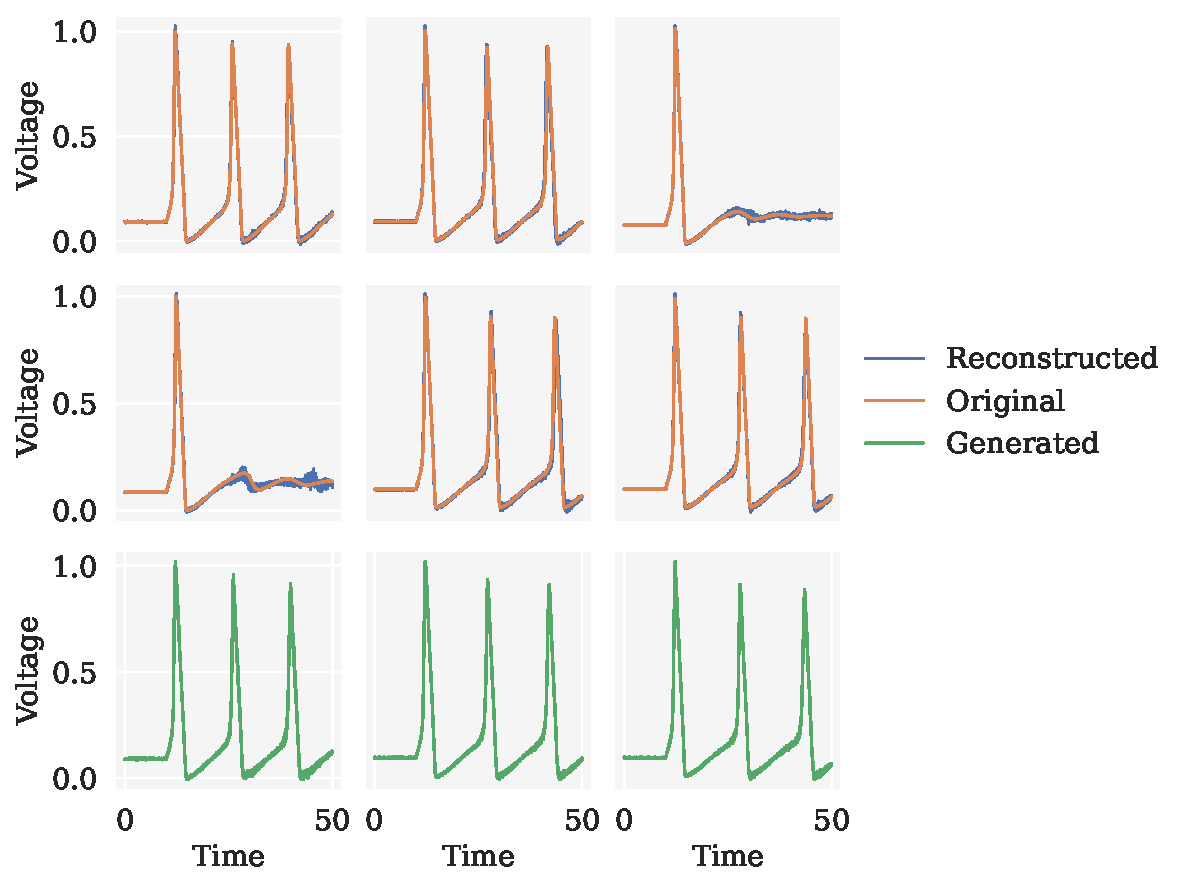
\includegraphics[scale=0.38]{latex/figures/hh_conv_vae_beta_2_z_2.pdf}}}
\qquad
\subfloat[]{{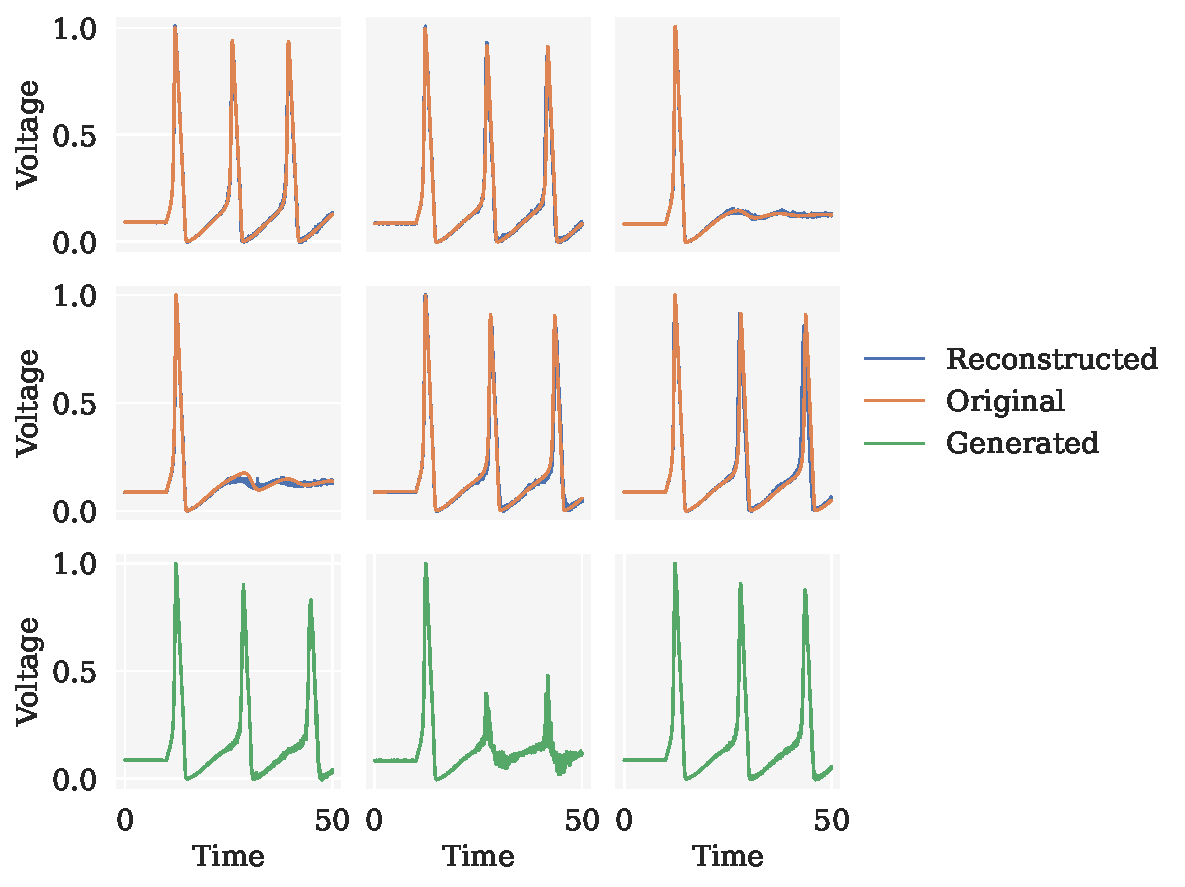
\includegraphics[scale=0.38]{latex/figures/hh_conv_vae_beta_2_z_10.pdf}}}
\qquad
\subfloat[]{{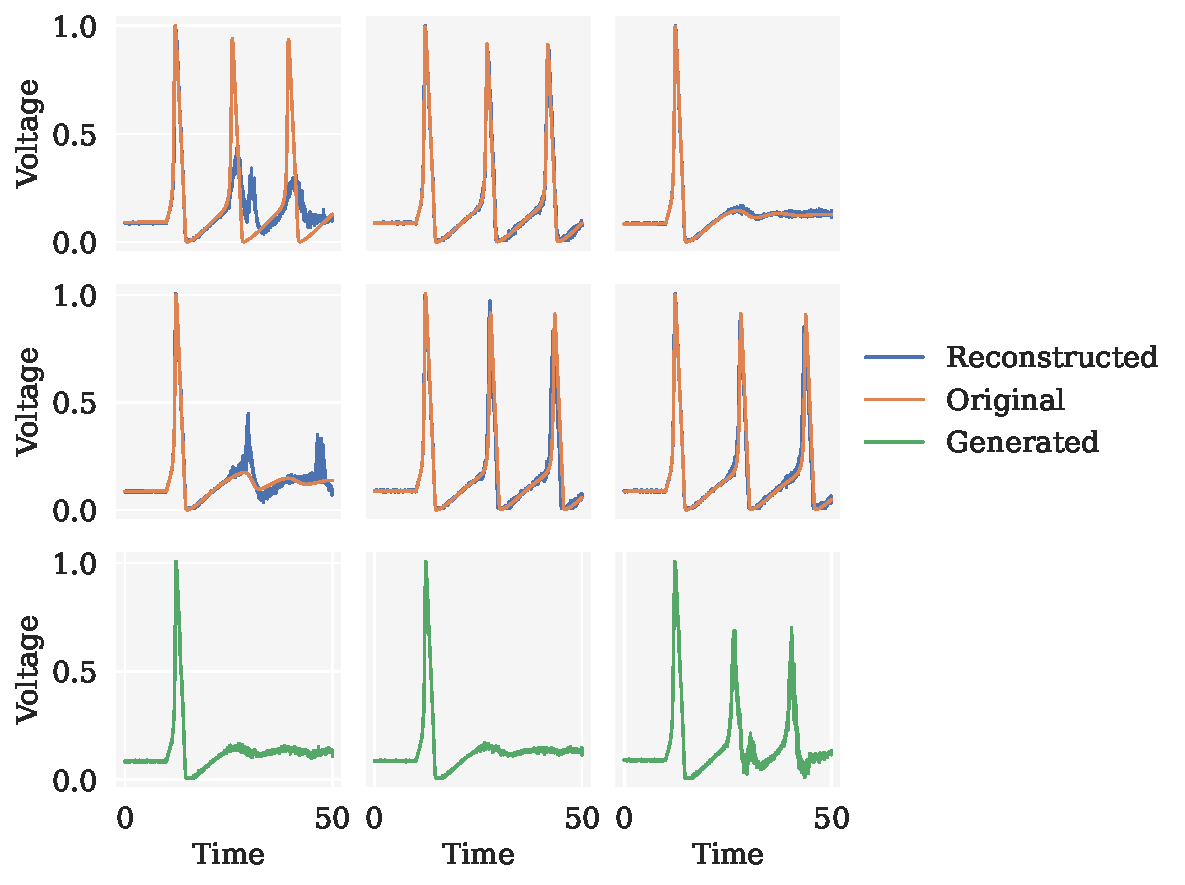
\includegraphics[scale=0.38]{latex/figures/hh_conv_vae_beta_2_z_20.pdf}}}
\caption{beta 2}
\label{fig:hh_conv_vae_beta_2}
\end{figure}
